\documentclass{article}

% if you need to pass options to natbib, use, e.g.:
% \PassOptionsToPackage{numbers, compress}{natbib}
% before loading nips_2018

% ready for submission
\usepackage[final]{nips_2018}

% to compile a preprint version, e.g., for submission to arXiv, add
% add the [preprint] option:
% \usepackage[preprint]{nips_2018}

% to compile a camera-ready version, add the [final] option, e.g.:
% \usepackage[final]{nips_2018}

% to avoid loading the natbib package, add option nonatbib:
% \usepackage[nonatbib]{nips_2018}

\usepackage[utf8]{inputenc} % allow utf-8 input
\usepackage[T1]{fontenc}    % use 8-bit T1 fonts
\usepackage{hyperref}       % hyperlinks
\usepackage{url}            % simple URL typesetting
\usepackage{booktabs}       % professional-quality tables
\usepackage{amsfonts}       % blackboard math symbols
\usepackage{amsmath}
\usepackage{nicefrac}       % compact symbols for 1/2, etc.
\usepackage{microtype}      % microtypography
\usepackage{graphicx}


\title{Project Milestone: arXiv vs. snarXiv}

\renewcommand{\P}{\mathbb{P}}
\newcommand{\V}{\mathcal{V}}

% The \author macro works with any number of authors. There are two
% commands used to separate the names and addresses of multiple
% authors: \And and \AND.
%
% Using \And between authors leaves it to LaTeX to determine where to
% break the lines. Using \AND forces a line break at that point. So,
% if LaTeX puts 3 of 4 authors names on the first line, and the last
% on the second line, try using \AND instead of \And before the third
% author name.

\author{Tyler Blanton \And Sam Kowash}
  %% examples of more authors
  %% \And
  %% Coauthor \\
  %% Affiliation \\
  %% Address \\
  %% \texttt{email} \\
  %% \AND
  %% Coauthor \\
  %% Affiliation \\
  %% Address \\
  %% \texttt{email} \\
  %% \And
  %% Coauthor \\
  %% Affiliation \\
  %% Address \\
  %% \texttt{email} \\
  %% \And
  %% Coauthor \\
  %% Affiliation \\
  %% Address \\
  %% \texttt{email} \\


\begin{document}
% \nipsfinalcopy is no longer used

\maketitle

\begin{abstract}
  We give a brief update on our project to develop a classifier that can accurately distinguish between real arXiv \texttt{hep-th} abstracts and fake abstracts generated from a context-free grammar by the program snarXiv\footnote{\url{http://davidsd.org/2010/03/the-snarxiv/}}.
  Our progress consists of three major parts: obtaining large amounts of data in an efficient way, parsing the abstract text to prepare it for analysis, and implementing a simple classification algorithm -- a naive Bayes classifier using a bag-of-words model.
  We chose this extremely simple classifier to serve as a proof of concept, though it already outperforms humans (successful classification rate is $\sim$85\% vs. 57\% for humans).
\end{abstract}




\section{Introduction} \label{sec:intro}
The arXiv exposes its search API through a well-documented HTTP interface, but this has limitations in the context of our project as it is configured to find no more than 30000 results, and return no more than 2000 of them at a time.
We estimate that \texttt{hep-th} has $\sim$85000 articles, and we'd ideally use all of them, so we need a more robust data acquisition tool.
Fortunately, arXiv also furnishes an Open Archives Initiative Protocol for Metadata Harvesting (OAI-PMH) interface, which is better-suited to full-repository harvesting. We use the \texttt{pyoai} module\footnote{\url{https://github.com/infrae/pyoai}} to retrieve the full metadata set from \texttt{hep-th}, extract the abstract text from the returned XML structure, and feed it to the parser, which normalizes it for analysis.

The snarXiv abstracts are even easier to obtain, since we can generate them at will.
We use a modified grammar file to produce only abstracts rather than titles and authors, then call the compiled snarXiv generator repeatedly to produce a corpus, which can be fed to the parser.
(The snarXiv generator could of course be modified to produce the desired format in the first place, but we prefer to use as much of the original tool as possible.)


\section{Implementation} \label{sec:implementation} % maybe should be in appendix
\subsection{Parsing abstract text}
The raw response from an arXiv API call is a bunch of text consisting of full \texttt{hep-th} papers (which often contain TeX symbols like \$ and  \textbackslash) along with several tags specifying sections as title, author, abstract, etc.
For simplicity, we are currently only focusing on the abstracts, which we pull out and organize into a list using Python's \texttt{feedparser} package.
We also store snarXiv abstracts in this form, so the rest of the parsing process is the same for the arXiv and snarXiv data.

The next step is to split the abstract text into regular words that are easily identifiable between different abstracts.
We split on all spaces and newlines, and for uniformity we make all words lowercase and strip out all punctuation.
This method works for the most part, but it leaves traces of some TeX commands; for example, it sends \texttt{\textbackslash mathbb\{Z\} $\to$ mathbbz}.
In the future we may try a more sophisticated approach where we deal with TeX commands at the beginning before stripping all punctuation, but for now this issue is only a minor nuisance.
In any case, the output of our parsing procedure is two lists of lists (one arXiv, one snarXiv), where each inner list is comprised of formatted words from a single abstract.


\section{Theory}
Each of the abstract classification algorithms we use consists of three main parts: a parser, a language model, and a classifier.
Here we discuss the theory behind our language models and classifiers; details about our parsing choices can be found in Section~\ref{sec:implementation}.
 
\subsection{Language models} \label{sec:LMs}
\subsubsection{$n$-grams}
Assume that each abstract $X$ has a probability $\P(X|Y)$ of being from source $Y\in\{-1,1\}$, where $Y=1$ represents the label ``snarXiv'' and  $Y=-1$ represents the label ``arXiv.''
Suppose $X=(w_1,w_2,\ldots,w_N)$ is an abstract containing $N$ words $\{w_i\}_{i=1}^N$, and let $w_i^{i+k}$ denote the word sequence $(w_i,w_{i+1},\ldots, w_{i+k})$.
The $n$-grams language model approximates $\P(X|Y)$ as
\begin{align}
	\P(X|Y) = \P(w_1^N|Y) &= \prod_{i=1}^N \P(w_i|w_1^{i-1},Y)
	\\
	&\approx \prod_{i=1}^N \P(w_i| w_{i-n+1}^{i-1},Y) \quad\; (n\text{-grams approx.})
\end{align}
In other words, in the $n$-grams model we assume that the probability of a given word $w$ occurring in some abstract only depends on what the previous $n-1$ words in the abstract are, where $n$ is some (typically small) positive integer; the $n-1$ words on which $w$ depends are called the ``context'' of $w$.

In the simplest case $n=1$, each word occurrence is assumed to be completely independent of any context, which is why the 1-gram language model is often referred to as the ``bag-of-words'' (BoW) model.
Given some training set of abstracts from source $Y$, we define our BoW training estimate $\widehat\P(X|Y)_\text{BoW}$ as
\begin{align}
  \widehat\P(X|Y)_\text{BoW} &=  \widehat\P(w_1^N|Y)_\text{BoW} \equiv \prod_{i=1}^N \widehat\P(w_i|Y), \\
  \text{where } \quad \widehat\P(w_i|Y) &\equiv \frac{C_Y(w_i)+1}{\sum_w [C_Y(w)+1]} = \frac{C_Y(w_i)+1}{\sum_{w\in\V} C_Y(w)+V},
\end{align}
$C_Y(w_i)$ is the number of times that $w_i$ appears, $\V$ is a vocabulary of size $V=|\V|$ containing all of the words that we wish to learn about, and $\sum_{w\in\V} C_Y(w)$ is the total number of words in the training set.
The extra $+1$ on each word count $C_Y(w)$ comes from Laplace smoothing, which is a precautionary measure taken to prevent zero probabilities from occurring in cases where we need to classify an abstract that contains a word that did not appear in the training set.
Other technical details regarding bag-of-words and $n$-grams implementation can be found in Appendix~\ref{app:details}. 

The generalization to $n>1$ is straightforward: we define our estimate $\widehat\P(X|Y)_{n\text{-gram}}$ for a given training set from source $Y$ to be
\begin{align}
	\widehat\P(X|Y)_{n\text{-gram}} = \widehat\P(w_1^N|Y)_{n\text{-gram}} &\equiv \prod_{i=1}^N \widehat\P(w_i| w_{i-n+1}^{i-1},Y),
	\\
	\text{where } \quad \widehat\P(w_i|w_{i-n+1}^{i-1},Y) &\equiv \frac{C_Y(w_{i-n+1}^i)+1}{C_Y(w_{i-n+1}^{i-1})+V},
\end{align}
$C_Y(w_{i-n+1}^i)$ is the number of times that the $n$-gram $w_{i-n+1}^i$ occurs, and $C_Y(w_{i-n+1}^{i-1})$ is the number of times that the $(n-1)$-gram $w_{i-n+1}^{i-1}$ appears.




\subsubsection{tf--idf}







\subsection{Classifiers}
\subsubsection{Naive Bayes classifier}
Our first attempt at creating a program that distinguishes between arXiv and snarXiv abstracts utilized a naive Bayes (NB) classifier.
The theory behind this classifier is simple: if $\P(Y=1|X) > \P(Y=-1|X)$, then we classify $X$ as snarXiv; otherwise, we classify it as arXiv.
We can use Bayes' theorem $\P(Y|X) = \frac{\P(Y)\P(X|Y)}{\P(X)}$ to rewrite this classification condition as
\begin{align}
	\widehat{Y}_{NB} \equiv \arg\max_{Y\in\{-1,1\}} \P(Y)\P(X|Y). \label{eq:Bayes}
\end{align}
We estimate each probability in \eqref{eq:Bayes} by training on a large number of arXiv and snarXiv abstracts.
We define our estimate%
\footnote{The probabilities $\P(Y=\pm1)$ are somewhat trivial since we generate the snarXiv abstracts ourselves and can control over how many arXiv vs. snarXiv abstracts will be in the train and test sets. Since the snarXiv was originally created to make abstracts that compete one-on-one with arXiv abstracts, we chose to set $\P(Y=\pm1)=\tfrac{1}{2}$ for all tests reported in this paper.}
%
for $\P(Y)$ as the number of abstracts in training set $Y$ over the total number of abstracts in both the arXiv and snarXiv training sets.
The conditional probabilities $\P(X|Y)$ are more complicated, and are approximated using a language model from Section~\ref{sec:LMs}.



\subsubsection{Likelihood-ratio test}
A slightly more sophisticated classification rule is the likelihood-ratio (LR) test.
For a given abstract $X$, define the likelihood ratio $\Lambda(X)\equiv\frac{\P(X|Y=1)}{\P(X|Y=-1)}$.
While we certainly want our classifier to correctly label all snarXiv abstracts as fakes, we also want to minimize the probability that an arXiv abstract gets incorrectly classified as fake.
The Neyman-Pearson lemma states that the optimal classifier
\begin{align}
	\delta_{LR}^* \equiv \arg\max_\delta \P(\delta(X)=1|Y=1), \text{\; subject to \;} \P(\delta(X)=1|Y=-1)\leq \alpha
\end{align}
for any fixed false-positive tolerance $\alpha$ takes the form
\begin{align}
	\P\left(\delta_{LR}^*(X)=1\right) =
	\begin{cases}
		1, 	& \Lambda(X) > \eta \\
		\gamma, & \Lambda(X) = \eta \\
		0, 	& \Lambda(X) < \eta,
	\end{cases}
\end{align}
where $\eta$ and $\gamma$ can be treated as hyperparameters to be tuned in cross-validation.
In practice, $\gamma$ is almost completely irrelevant since for any $\eta$, the odds that a language model like $n$-grams would yield an estimate for $\Lambda(X)$ that is \textit{exactly} equal to $\eta$ are essentially zero.%
\footnote{The borderline case of the naive Bayes classifier where $\P(Y=\pm1|X)=\frac{1}{2}$ is irrelevant for the same reason.}
%
We arbitrarily use $\gamma=0.5$, meaning the only hyperparameter we tune is $\eta$.











\section{Results}

Testing the method on new abstracts after training on 800 arXiv and 800 snarXiv abstracts, we find that the algorithm correctly classifies an abstract as arXiv or snarXiv roughly 85\% of the time.
This accuracy is not fantastic (which is to be expected given the simplicity of the model), but it is higher than we expected, and is already well higher than the average human classification accuracy of 57\%.%
\footnote{According to \url{http://snarxiv.org/vs-arxiv/highscores/}}
Looking a little more closely at the results, we find that the only misclassifications made are arXiv abstracts that the classifier mistakes as snarXiv -- when a snarXiv abstract is tested, it is correctly identified as snarXiv 100\% of the time.
The explanation for this finding is relatively simple: snarXiv only has about 1000 unique words that it pulls from when generating fake abstracts, so each of these words occurs with a significant probability.
Any reasonably large training set exposes this, and thus the classifier has no problem identifying snarXiv abstracts correctly.
On the other hand, 800 arXiv abstracts contain roughly 6000 unique words (making for lower individual word probabilities), and thus the classifier can struggle when an arXiv abstract contains several snarXiv words.




\begin{figure}[!htbp]
\centering
	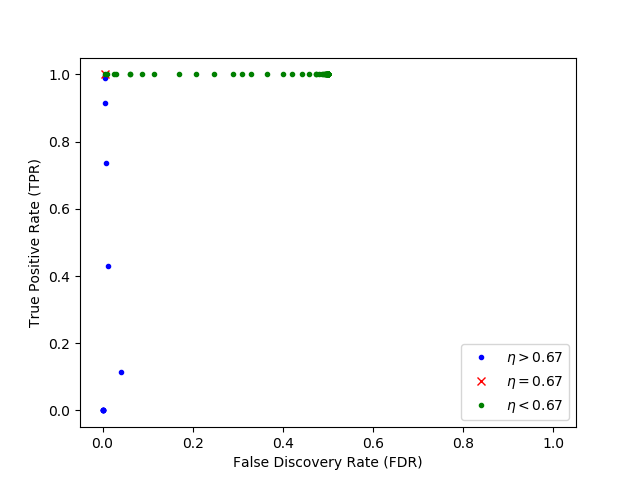
\includegraphics[width=0.48\textwidth]{../figures/FDR_TPR_plot.png}
	%\caption{LR-classifier using bag-of-words model.}
\end{figure}



\begin{figure}[!htbp]
\centering
	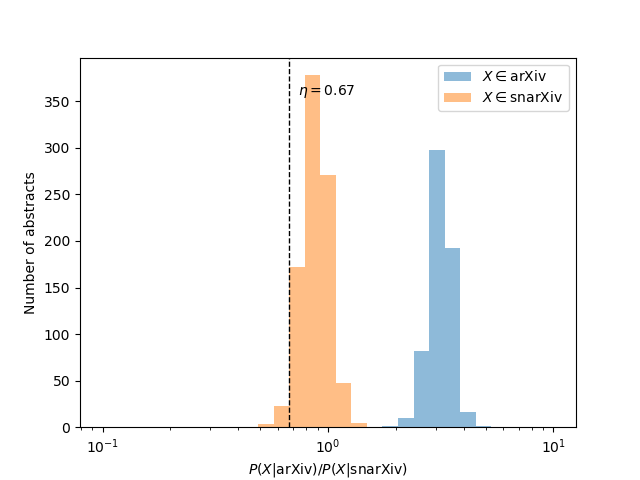
\includegraphics[width=0.48\textwidth]{../figures/BOW_histogram.png}
	%\caption{LR-classifier using bag-of-words model.}
	\hfill
	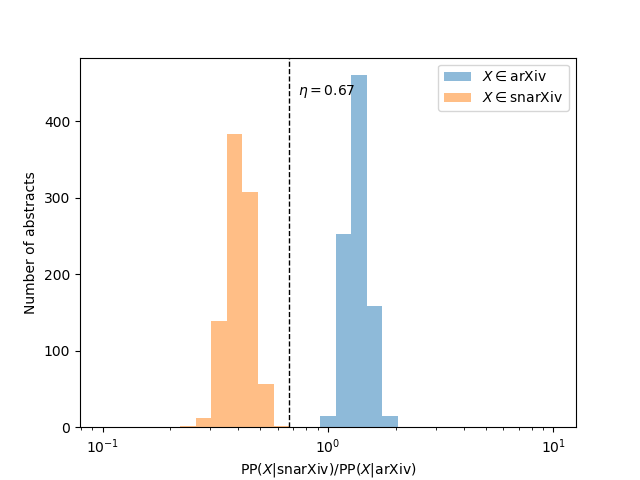
\includegraphics[width=0.48\textwidth]{../figures/bigram_histogram.png}
	%\caption{LR-classifier using bigram model.}
\end{figure}




















\section{Conclusions}
\subsection{Feature development}
Currently, our feature model represents a given abstract as a dictionary of occurrence counts for each word in the abstract and each word known from the training corpus.
This is called a bag-of-words model and is completely insensitive to word order, meaning that it is impossible for a classifier to take into account word co-occurrence rates or sentence position, which obviously contain most of the information in natural language.
(That our simple classification scheme achieves such reasonable performance given an extremely reductive model is surprising, and might suggest that the problem as posed is too easy; more thoughts on that below.)

The next step from a context-insensitive model is, obviously, the incorporation of context: instead of looking at how many times a given word appears in an abstract, we can look at the number of times it appears adjacent to each other word, or the number of times it appears in a triad with each pair of other words. This leads generically to the class of $n$-gram models, which incorporate length-$n$ sequences of words as elementary objects of analysis.

Concretely, the Brown model is a common framework in which language production is treated as a Markov process with hidden states and transition probabilities, and frames the learning task as estimating these properties from $n$-gram occurrence data in the corpus.
This task is complicated, however, by the rapidly ballooning amount of data that is produced if we must account for the occurrence of \emph{every} possible $n$-gram, even considering relatively small maximum correlation lengths.
This leads naturally to the field of word embeddings, which aim to map this painfully high-dimensional space into a lower-dimensional feature space in a way that preserves useful information about relationships between words from the $n$-gram structure.
\citet{stratos2015model} and \citet{stratos2014spectral} discuss efficient methods for generating embeddings from corpora, which will be our next implementation step in feature design.














\subsection{Possible extension}
Our results thus far suggest that the language produced by snarXiv may just be too artificial and constrained to put up much of a fight in the classification task.
The naive Bayes classifier never mistakes a snarXiv paper for real, although it still accidentally flags a decent chunk of real papers as fake.
We will continue this work with more sophisticated feature generation and classifiers to explore different methods and try to reduce the remaining error, but it is worth looking in other directions as well.

In particular, if snarXiv cannot produce abstracts that are convincing to our classifier, what can?
The field of generative adversarial networks has become prominent recently, as reviewed in \citet{creswell2018generative}, and we are considering extending our project in this direction.
The aim would be to produce, effectively, a next-generation snarXiv that achieves a meaningful error rate against its discriminating counterpart.
Several sources note that GANs are not naturally suited to contexts with discrete data streams, so this may prove unworkable, but is one direction to pursue if our original plan leads to shallow results.





\appendix
\section{Technical details} \label{app:details}
\subsection{Parsing abstract text}
Our parser attempts to translate the raw abstract text (a string) to a list of formatted words that are easily identifiable between different abstracts.
We first split the text on all spaces, newlines, and hyphens, and for uniformity we make all words lowercase.
Next, we look for words that end in a period or question mark and insert the special word tokens \texttt{<e>} and \texttt{<s>} afterwards to mark the end of one sentence and the start of another.
Lastly, we strip out all punctuation (except for the special tokens), prepend \texttt{<s>} to the list (marking the start of the first sentence), and delete the last word if the list ends \texttt{<e>} \texttt{<s>} (otherwise, we append \texttt{<e>}).

An example of parser input/output is

Input: \texttt{``I'm taking a CSE class on machine-learning.\ It's a lot of work, but pretty interesting.''}

Output: \texttt{[<s>, im, taking, a, cse, class, on, machine, learning, <e>, <s>, its, a, lot, of, work, but, pretty, interesting, <e>]}, 

where each ``word'' in the output list is a string.

Our parsing scheme works well, but it leaves traces of some TeX commands from the raw abstract text; for example, it sends \texttt{\textbackslash mathbb\{Z\} $\to$ mathbbz}.
This would be fine if all arXiv and snarXiv abstracts have TeX commands written the same way, though it is possible in some cases for abstracts to write the same command in different ways. In practice, we find that these instances are rare enough for the concern to be negligible.


\subsection{Vocabulary}
We defined our vocabulary $\V$ as the collection of $V=15,315$ unique words that appeared at least twice in a training corpus of 12,000 randomly chosen parsed arXiv abstracts and 12,000 (randomly generated) parsed snarXiv abstracts.
We decided not to include the 13,960 words that only appeared once since they seem to be relatively uncommon (often they are the residuals of TeX commands), and including them would nearly double our vocabulary size.
This pruning can be thought of as a feature-processing step.


\subsection{$n$-grams}
It is fairly common for a word to appear in the test set that is not in the vocabulary.
When this happens, we change the word to a special token \texttt{<UNK>}.
We then treat \texttt{<UNK>} as we would any other word when counting $n$-gram occurrences $C_Y(\cdot)$.

We prepend copies of the start sentence token \texttt{<s>} to each parsed abstract to ensure that the first $n$-gram consists of $n-1$ copies of \texttt{<s>} and one ``real'' word.
Similarly, we append copies of \texttt{<e>} to the end of each parsed abstract.

\subsection{Managing probabilities numerically}
Consider an abstract $X$ from source $Y$.
A typical arXiv/snarXiv abstract contains roughly 100 words, so the abstract probability $\P(X|Y)=\prod_{i=1}^N \P(w_i|w_1^{i-1},Y)$ is a product of $N\approx100$ different word probabilities, each of which is typically much less than one.
As a result, the size of $\P(X|Y)$ is heavily dependent on the abstract length and is usually extremely small, easily hitting numerical underflow in some cases.
To combat the issue of length dependence, we prefer to work with the perplexity
\begin{align}
	\text{PP}(X|Y) \equiv \sqrt[N]{\frac{1}{\P(X|Y)}} = \left[ \prod_{i=1}^N \P(w_i|w_1^{i-1},Y) \right]^{-1/N},
\end{align}
which normalizes the abstract probability by taking the geometric mean of the individual word probabilities (and inverting).
To prevent numerical underflow from rendering our algorithms useless, we always work with logs of probabilities in our code, which turns products into sums and keeps the numbers reasonable.
Note that the log of the perplexity is a simple arithmetic mean:
\begin{align}
	\log\text{PP}(X|Y) = -\frac{1}{N}\log\P(X|Y) = -\frac{1}{N} \sum_{i=1}^N \log\P(w_i|w_1^{i-1},Y).
\end{align}







\nocite{*}

\bibliographystyle{plainnat}
\bibliography{references}
\end{document}
